\chapter{Экспериментальный раздел}
\label{cha:research}

\section{Примеры работы}
На рисунке \ref{fig:4.1} приведен пример работы программы.

\begin{figure}[h]
    \centering
    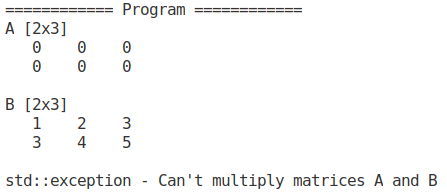
\includegraphics[width=0.6\textwidth]{2/inc/e1.png}
    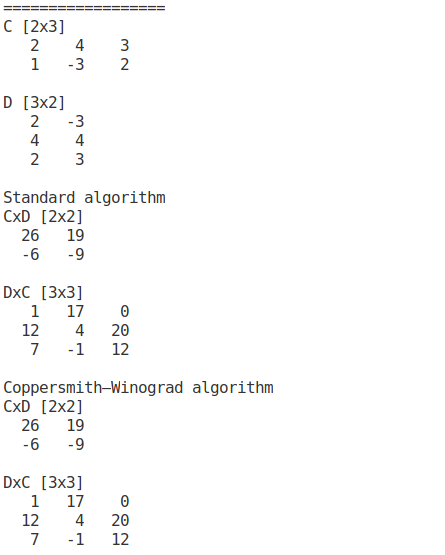
\includegraphics[width=0.6\textwidth]{2/inc/e2.png}
    \caption{Примеры работы алгоритмов умножения матриц}
    \label{fig:4.1}
\end{figure}


\pagebreak
\section{Результаты тестирования}

На рисунке \ref{fig:4.2} приведен результат теста с использованием фреймворка google test.

\begin{figure}[h]
    \centering
    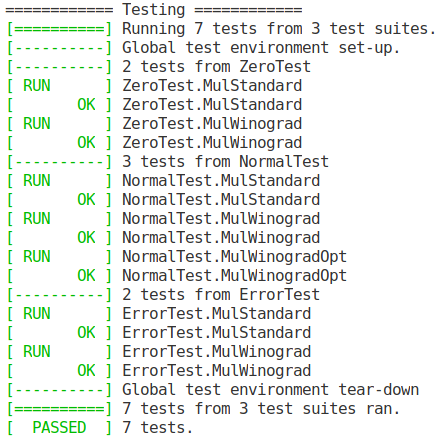
\includegraphics[width=0.6\textwidth]{2/inc/test.png}
    \caption{Примеры работы алгоритмов умножения матриц}
    \label{fig:4.2}
\end{figure}


% \section{Постановка эксперимента по замеру времени}
\section{Сравнение времени работы}

В таблице \ref{tabular:benchmark} приведены замеры времени
работы алгоритмов умножения матриц на квадратных матрицах,
на основе них построены графики \ref{fig:4.3} и \ref{fig:4.4}.

%  приведен функциональные тесты для алгоритмов
% вычисления расстояния Левенштейна и Дамерау — Левенштейна.


\def\arraystretch{1.2}
% \setlength\tabcolsep{0.2cm}

\pagebreak
\begin{table}[h]
    \centering
    \csvreader[tabular=|c|c|c|c|,
        table head=\hline
        \bfseries Размер
        & \bfseries Стандартный
        & \bfseries Винограда
        & \bfseries Винограда(о)
        \\\hline,
        late after line=\\\hline]
        {2/inc/benchmark1.csv}{}
    { \csvcoli & \csvcolii & \csvcoliii & \csvcoliv}
    \csvreader[tabular=|c|c|c|c|,
        table head=\hline
        \bfseries Размер
        & \bfseries Стандартный
        & \bfseries Винограда
        & \bfseries Винограда(о)
        \\\hline,
        late after line=\\\hline]
        {2/inc/benchmark2.csv}{}
    { \csvcoli & \csvcolii & \csvcoliii & \csvcoliv}
    % \csvautotabular{2/inc/benchmark2.csv}
    \caption{\label{tabular:benchmark} Времени работы (ns)}
\end{table}

% \clearpage
\pagebreak
\begin{figure}[!h]
    \centering
    \begin{tikzpicture}
        \begin{axis}[
            scale=1.4,
            axis lines=left,
            xlabel=Размер матрицы,
            ylabel={Время, нс},
            legend pos=north west,
            xmajorgrids=true,
            ymajorgrids=true
        ]
            \addplot table[x=n,y=t1,col sep=comma] {2/inc/benchmark1.csv};
            \addplot table[x=n,y=t2,col sep=comma] {2/inc/benchmark1.csv};
            \addplot table[x=n,y=t3,col sep=comma] {2/inc/benchmark1.csv};
            \legend{Стандартный, Винограда, Винограда(о)}
        \end{axis}
    \end{tikzpicture}
    \caption{Зависимость времени работы алгоритмов умножения матриц от размеры матрицы (при четном размере)}
    \label{fig:4.3}
\end{figure}


\begin{figure}[!h]
    \centering
    \begin{tikzpicture}
        \begin{axis}[
            scale=1.4,
            axis lines=left,
            xlabel=Размер матрицы,
            ylabel={Время, нс},
            legend pos=north west,
            xmajorgrids=true,
            ymajorgrids=true
        ]
            \addplot table[x=n,y=t1,col sep=comma] {2/inc/benchmark2.csv};
            \addplot table[x=n,y=t2,col sep=comma] {2/inc/benchmark2.csv};
            \addplot table[x=n,y=t3,col sep=comma] {2/inc/benchmark2.csv};
            \legend{Стандартный, Винограда, Винограда(о)}
        \end{axis}
    \end{tikzpicture}
    \caption{Зависимость времени работы алгоритмов умножения матриц от размеры матрицы (при нечетном размере)}
    \label{fig:4.4}
\end{figure}

% \section{Сравнительный анализ на материале экспериментальных данных}
% эксперименты+выводы

\section{Вывод}

Из графики, очевидно, что алгоритм Винограда с оптимизацией самый быстрый,
на матрицах размером 800x800 работает примерно на 20\% (15-25\% зависит от m четное или нечетное)
быстрее стандартный алгоритм.
